\documentclass[12pt,a4paper,twoside]{article}
\input{185.dat}
\usepackage{gensymb}
\usepackage{amsthm}
\usepackage{float}
\usepackage{siunitx}
\usepackage{amssymb}
\usepackage{float}
\usepackage{enumerate}
\usepackage{listings}
\usepackage{mathtools}
\usepackage[none]{hyphenat}
\usepackage{physics}
\newcommand\ddfrac[2]{\frac{\displaystyle #1}{\displaystyle #2}}
%\renewcommand{\familydefault}{\sfdefault}
\usepackage{booktabs,tabularx}
\usepackage{tabulary}
\renewcommand{\tabularxcolumn}{m}
\usepackage{listings}
\PassOptionsToPackage{hyphens}{url}\usepackage{hyperref}
\usepackage{color, colortbl}
\definecolor{cyan}{rgb}{0.85,0.89,0.95}
\renewcommand{\familydefault}{\sfdefault}

\begin{document}

\begin{titlepage}
\begin{center}
\vspace*{\fill}

\Huge{ Live-Feed-over-LAN Pressure Sensor (LoLAN-PresS) Documentation} \\

\qquad
\qquad

\normalsize{Members: \\ 
Kenneth V. Domingo \\
Rhei Joven G. Juan \\
Rene L. Principe Jr. \\ \medskip
App Physics 185 }

\vspace*{\fill}
\end{center}
\end{titlepage}

\setcounter{page}{1}

\section{Overview}\label{sec:overview}
\medskip
The Live-Feed-over-LAN Pressure Sensor (LoLAN-PresS) is an implementation of velostat pressure/bend sensor which runs on an ESP8266-based microcontroller. On the hardware end, the sensor broadcasts through a local area network (LAN) using a pre-set IP address. On the software end, the feed can be retrieved, processed, and displayed in real-time through any Python interpreter on a device connected on the same network. The program depends on the following Python libraries:

\begin{itemize}

\item Numpy
\item Matplotlib
\item Scipy
\item URLlib

\end{itemize}

\section{Hardware setup}\label{sec:hardware}\medskip
The hardware of LoLAN-PresS requires the following items along with their costs during Q2 2019:

\begin{table}[h!]
	\centering
	\caption{Cost of required materials.}
	\begin{tabulary}{\linewidth}{CCCCC}
	Qty & Item & Source & Cost/pc (PhP) & Subtotal (PhP) \\ \hline
	1 & Velostat sheet & circuit.rocks & 349.00 & 349.00 \\
	1 & NodeMCU 1.0 Lua WiFi Board & circuit.rocks & 325.00 & 325.00 \\
	& & & \textbf{TOTAL} & 674.00
	\end{tabulary}
\end{table}

The velostat may come in small patches or a large sheet. Cutting this into the desired shape results in little change in its properties. 

\begin{figure}[h!]
	\centering
	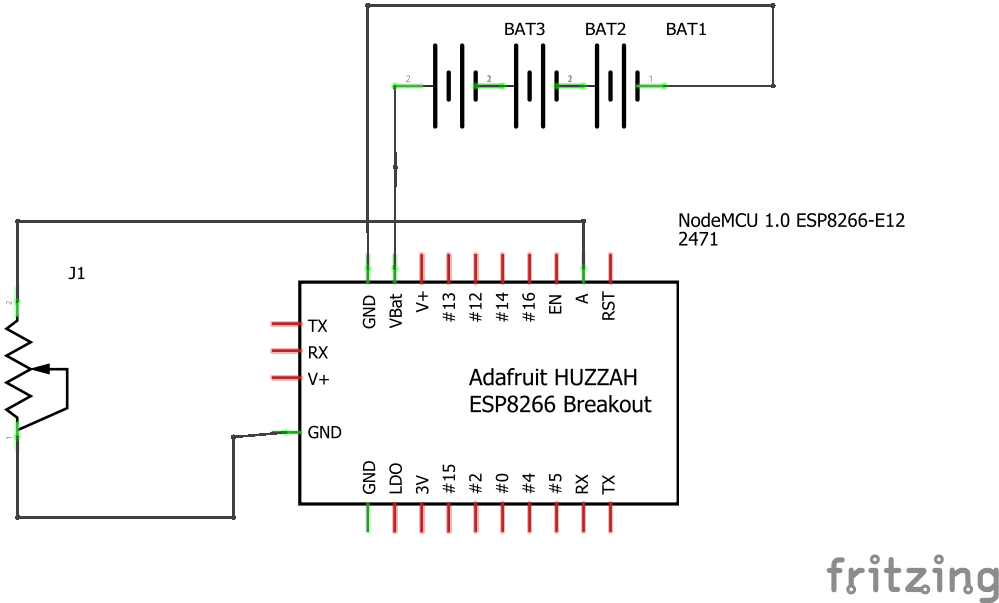
\includegraphics[width=0.75\linewidth]{setup.png}
	\caption{Schematic of the hardware setup.}
	\label{fig:schematic}
\end{figure}

\section{Software setup}\label{sec:software}\medskip

\subsection{The \texttt{PressureSensor} class}
The \texttt{PressureSensor} class contains the functions and attributes needed for communication with the microcontroller and live display of the analog data.

\subsubsection{\texttt{\footnotesize{PressureSensor}\normalsize{.\_\_init\_\_(url, calibration)}}}
Instantiates the \texttt{Spectrometer} object and takes the calibration arguments.

\begin{table}[H]
    \caption{Program initialization.}
    \begin{tabular}{>{\columncolor{cyan}}p{2in} p{4in}}
        \hline
        \textbf{Parameters} & \texttt{url : str} \\
        &   Local IP address of the microcontroller. \\ 
        & \texttt{calibration : str} \\
        &   Filename of the data to be used for calibration of voltage-to-force. \\ \hline
    \end{tabular}
    \label{tab:prog-init}
\end{table}

\subsubsection{\texttt{\footnotesize{PressureSensor}\normalsize{.plot\_calibration()}}}
Displays the calibration curve and the voltage-to-force equation.

\subsubsection{\texttt{\footnotesize{PressureSensor}\normalsize{.runlive()}}}
Starts the live feed and saves all currently received data every 3 seconds to \texttt{datalog.npy}.

\subsection{The \texttt{characterization} class}
The \texttt{characterization} class allows the retrieval and processing of saved \texttt{.npy} files for processing later on.

\subsubsection{\texttt{\footnotesize{characterization}\normalsize{.\_\_init\_\_(filename, width, polyorder, lim)}}}
Instantiates the \texttt{Spectrometer} object.

\begin{table}[H]
    \caption{Program initialization.}
    \begin{tabular}{>{\columncolor{cyan}}p{2in} p{4in}}
        \hline
        \textbf{Parameters} & \texttt{filename : str} \\
        &   Filename of the data to be processed. Accepts \texttt{.txt}, \texttt{.log}, and \texttt{.npy} formats. \\ 
        & \texttt{width : int} \\
        &   Specifies the filter window length of the Savitzky-Golay filter. \\ 
        & \texttt{polyorder : int} \\
        &	Specifies the order of the polynomial used to fit the samples in the Savitzky-Golay filter. \\
        & \texttt{lim : tuple} \\
        &	Specifies the index range of the data to be processed. \\ \hline
    \end{tabular}
    \label{tab:prog-characterize}
\end{table}

The full code is available in the Appendix.

\section{Demonstration}



\section*{Appendix}
Source code:

%\bibliographystyle{spp-bst}
%\bibliography{bibfile}

%\raggedbottom

%\pagebreak
%\pagebreak[3]
\iffalse
\newpage

\renewcommand\thefigure{A\arabic{figure}} 
\setcounter{figure}{0}
\fi %removing this will break the code for some reason

\end{document}

